% Compile this file in Overleaf with pdfLaTeX.
% Keep cu-logo.png in the same Overleaf project as this file.
% Replace the editable details below before final submission.

\documentclass[12pt,a4paper,oneside]{report}

\usepackage[a4paper,left=1.5in,right=1in,top=1in,bottom=1in]{geometry}
\usepackage[T1]{fontenc}
\usepackage[utf8]{inputenc}
\usepackage{newtxtext,newtxmath} % Times New Roman compatible font
\usepackage{setspace}
\usepackage{ragged2e}
\usepackage{titlesec}
\usepackage{tocloft}
\usepackage{graphicx}
\usepackage{booktabs}
\usepackage{tabularx}
\usepackage{array}
\usepackage{enumitem}
\usepackage{caption}
\usepackage{pgfgantt}
\usepackage{tikz}
\usetikzlibrary{arrows.meta,positioning,shapes.geometric}
\usepackage{url}
\usepackage[hidelinks]{hyperref}

% The references page is intentionally omitted in this version.
\renewcommand{\cite}[1]{}

% -----------------------------------------------------------------------------
% EDITABLE PROJECT DETAILS
% -----------------------------------------------------------------------------
\newcommand{\projecttitle}{AI HIRING INTELLIGENCE PLATFORM}
\newcommand{\studentone}{STUDENT NAME (UID)}
\newcommand{\studenttwo}{SECOND STUDENT NAME (UID)} % Delete if not required
\newcommand{\degree}{BACHELOR OF ENGINEERING}
\newcommand{\branch}{COMPUTER SCIENCE \& ENGINEERING}
\newcommand{\department}{Department of Computer Science and Engineering}
\newcommand{\hodname}{NAME OF THE HEAD OF DEPARTMENT}
\newcommand{\supervisorname}{NAME OF THE SUPERVISOR}
\newcommand{\supervisordesignation}{ACADEMIC DESIGNATION}
\newcommand{\submissionmonth}{JULY 2026}
\newcommand{\vivadate}{DD/MM/YYYY}

% -----------------------------------------------------------------------------
% UNIVERSITY FORMAT
% -----------------------------------------------------------------------------
\onehalfspacing
\justifying
\setlength{\parindent}{0.5in}
\setlength{\parskip}{0pt}

% Chapter: 16 pt, bold, centered. Heading: 14 pt, bold, left aligned.
\titleformat{\chapter}[display]
  {\normalfont\bfseries\centering\fontsize{16}{19}\selectfont}
  {CHAPTER \thechapter}{6pt}{\MakeUppercase}
\titlespacing*{\chapter}{0pt}{-20pt}{18pt}

\titleformat{\section}
  {\normalfont\bfseries\fontsize{14}{17}\selectfont}
  {\thesection.}{0.6em}{}
\titlespacing*{\section}{0pt}{0pt}{8pt}

\titleformat{\subsection}
  {\normalfont\bfseries\fontsize{12}{15}\selectfont}
  {\thesubsection.}{0.6em}{}

\captionsetup{font={small,bf},labelfont=bf}
\renewcommand{\cftchapfont}{\bfseries}
\renewcommand{\cftchappagefont}{\bfseries}
\setcounter{tocdepth}{2}
\setcounter{secnumdepth}{3}

\newcommand{\culogo}{%
  
\includegraphics[width=0.48\textwidth]{cu-logo.png}}

\begin{document}

% -----------------------------------------------------------------------------
% TITLE PAGE
% -----------------------------------------------------------------------------
\begin{titlepage}
\begin{center}
{\bfseries\fontsize{18}{22}\selectfont \projecttitle\par}
\vspace{1.0cm}
{\bfseries\fontsize{14}{17}\selectfont A PROJECT REPORT\par}
\vspace{1.3cm}
{\bfseries\itshape\fontsize{14}{17}\selectfont Submitted by\par}
\vspace{0.7cm}
{\bfseries\fontsize{16}{19}\selectfont \studentone\par}
{\bfseries\fontsize{16}{19}\selectfont \studenttwo\par}
\vspace{1.1cm}
{\bfseries\itshape\fontsize{14}{18}\selectfont
in partial fulfillment for the award of the degree of\par}
\vspace{0.8cm}
{\bfseries\fontsize{16}{19}\selectfont \degree\par}
\vspace{0.4cm}
{\bfseries\fontsize{14}{17}\selectfont IN\par}
\vspace{0.35cm}
{\fontsize{14}{17}\selectfont \branch\par}
\vfill
\culogo
\vspace{0.3cm}

{\bfseries\fontsize{14}{17}\selectfont Chandigarh University\par}
\vspace{0.4cm}
{\fontsize{14}{17}\selectfont \submissionmonth\par}
\end{center}
\end{titlepage}

% -----------------------------------------------------------------------------
% BONAFIDE CERTIFICATE
% -----------------------------------------------------------------------------
\clearpage
\thispagestyle{empty}
\begin{center}
\culogo
\vspace{0.7cm}

{\bfseries\fontsize{16}{19}\selectfont BONAFIDE CERTIFICATE}
\end{center}

\vspace{1.0cm}
\begin{spacing}{2}
\fontsize{14}{20}\selectfont
\noindent Certified that this project report entitled ``\textbf{\projecttitle}'' is the
bonafide work of \textbf{\studentone} and \textbf{\studenttwo}, who carried out the
project work under my supervision.
\end{spacing}

\vspace{1.2cm}
\noindent
\begin{minipage}[t]{0.46\textwidth}
\textbf{SIGNATURE}\\[0.65cm]
\hodname\\
\textbf{HEAD OF THE DEPARTMENT}\\
\department
\end{minipage}
\hfill
\begin{minipage}[t]{0.46\textwidth}
\textbf{SIGNATURE}\\[0.65cm]
\supervisorname\\
\textbf{SUPERVISOR}\\
\supervisordesignation\\
\department
\end{minipage}

\vfill
\noindent Submitted for the project viva-voce examination held on \vivadate.

\vspace{1.1cm}
\noindent
\textbf{INTERNAL EXAMINER}
\hfill
\textbf{EXTERNAL EXAMINER}

% -----------------------------------------------------------------------------
% ACKNOWLEDGEMENT AND CONTENT LISTS
% -----------------------------------------------------------------------------
\clearpage
\pagenumbering{roman}
\chapter*{ACKNOWLEDGEMENT}
\addcontentsline{toc}{chapter}{Acknowledgement}
We express our sincere gratitude to our project supervisor, \supervisorname, for
continuous guidance, constructive suggestions, and encouragement throughout this
project. We also thank the Head and faculty members of \department, Chandigarh
University, for providing the academic environment and resources required to
complete the work. We are grateful to our peers and families for their support and
valuable feedback. Finally, we acknowledge the researchers, standards bodies, and
open-source communities whose publications and software tools supported the design,
implementation, and evaluation of the AI Hiring Intelligence Platform.

\clearpage
\tableofcontents

\clearpage
\addcontentsline{toc}{chapter}{List of Figures}
\listoffigures

\clearpage
\addcontentsline{toc}{chapter}{List of Tables}
\listoftables

% -----------------------------------------------------------------------------
% ABSTRACT
% -----------------------------------------------------------------------------
\clearpage
\chapter*{ABSTRACT}
\addcontentsline{toc}{chapter}{Abstract}
\begin{spacing}{2}
% A 14 pt base leading doubled by the spacing environment gives 28 pt lines.
% This keeps the university's double-spacing rule while fitting one A4 page.
\fontsize{14}{14}\selectfont
Recruitment requires organizations to assess candidates consistently and make
decisions that can be explained. Conventional workflows often divide resumes,
interviews, coding exercises, reviewer notes, and reports across disconnected tools.
The \textbf{AI Hiring Intelligence Platform} was developed as a unified, multi-tenant
web application for structured technical hiring. It allows recruiters to define jobs
and skills, publish versioned assessments, invite candidates, conduct adaptive
interviews, evaluate coding and system-design work, and generate evidence-linked
reports. A separate candidate portal provides passwordless access, saved progress,
resume management, and privacy-request functions.

Resume intelligence is provided by CVerify, a locally served DistilBERT classifier
covering 24 job families. On a held-out test set, it achieved 86.35\% accuracy,
85.36\% weighted F1-score, and 79.47\% macro F1-score. The platform uses Next.js,
NestJS, PostgreSQL, Redis, FastAPI, and restricted Docker containers. Security
controls include separate recruiter and candidate sessions, role-based permissions,
organization-scoped data access, hashed tokens, immutable assessment snapshots, and
audit records. Artificial intelligence supports rather than replaces professional
judgement: outputs are validated, evidence is retained, and recommendations remain
reviewable. The project improves workflow consistency and traceability while
recognizing the need for human oversight, privacy governance, bias monitoring, and
field validation.

\noindent\textbf{Keywords:} artificial intelligence, recruitment, adaptive interview,
resume classification, DistilBERT, candidate assessment, explainable evaluation.
\end{spacing}

% -----------------------------------------------------------------------------
% GRAPHICAL ABSTRACT
% -----------------------------------------------------------------------------
\clearpage
\chapter*{GRAPHICAL ABSTRACT}
\addcontentsline{toc}{chapter}{Graphical Abstract}
\begin{center}
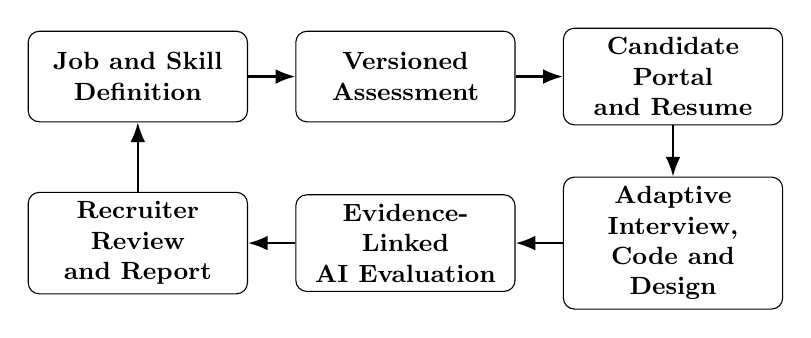
\begin{tikzpicture}[
  node distance=0.65cm and 0.6cm,
  box/.style={draw, rounded corners, align=center, minimum height=1.15cm,
              text width=2.55cm, font=\small\bfseries},
  arrow/.style={-{Latex[length=2.5mm]}, thick}
]
\node[box] (job) {Job and Skill\\Definition};
\node[box, right=of job] (assessment) {Versioned\\Assessment};
\node[box, right=of assessment] (candidate) {Candidate Portal\\and Resume};
\node[box, below=of candidate] (interview) {Adaptive Interview,\\Code and Design};
\node[box, left=of interview] (evaluation) {Evidence-Linked\\AI Evaluation};
\node[box, left=of evaluation] (report) {Recruiter Review\\and Report};
\draw[arrow] (job) -- (assessment);
\draw[arrow] (assessment) -- (candidate);
\draw[arrow] (candidate) -- (interview);
\draw[arrow] (interview) -- (evaluation);
\draw[arrow] (evaluation) -- (report);
\draw[arrow] (report) -- (job);
\end{tikzpicture}

\vspace{1cm}
\textbf{AI Hiring Intelligence Platform: human-supervised, evidence-based hiring workflow}
\end{center}

% -----------------------------------------------------------------------------
% ABBREVIATIONS AND SYMBOLS
% -----------------------------------------------------------------------------
\clearpage
\chapter*{ABBREVIATIONS}
\addcontentsline{toc}{chapter}{Abbreviations}
\begin{tabular}{>{\bfseries}p{0.22\textwidth}p{0.68\textwidth}}
AI & Artificial Intelligence \\
API & Application Programming Interface \\
ATS & Applicant Tracking System \\
JWT & JSON Web Token \\
NLP & Natural Language Processing \\
OCR & Optical Character Recognition \\
RBAC & Role-Based Access Control \\
REST & Representational State Transfer \\
SaaS & Software as a Service \\
UI & User Interface \\
\end{tabular}

\clearpage
\chapter*{SYMBOLS}
\addcontentsline{toc}{chapter}{Symbols}
\begin{tabular}{>{\bfseries}p{0.22\textwidth}p{0.68\textwidth}}
$P$ & Precision of a classifier \\
$R$ & Recall of a classifier \\
$F_1$ & Harmonic mean of precision and recall \\
$n$ & Number of observations or documents \\
$\%$ & Percentage \\
\end{tabular}

% -----------------------------------------------------------------------------
% CHAPTER 1
% -----------------------------------------------------------------------------
\clearpage
\pagenumbering{arabic}
\setcounter{page}{1}
\chapter{INTRODUCTION}

\section{Client Identification/Need Identification/Identification of Relevant Contemporary Issue}

The principal clients of this project are recruitment teams, hiring managers, and
technical interviewers in organizations that recruit candidates for skill-intensive
roles. These users must define job requirements, process applications, coordinate
assessments, compare evidence, and document decisions. Candidates are an equally
important stakeholder group because they provide sensitive information, complete the
assessment, and experience the consequences of the process. System administrators
form a third group responsible for access, security, service availability, and usage
governance.

The need exists because hiring requirements and available skills are changing rapidly.
The World Economic Forum's \textit{Future of Jobs Report 2025}, based on a survey of
more than 1,000 employers representing over 14 million workers across 55 economies,
reports that 39\% of workers' existing skill sets are expected to be transformed or
become outdated by 2030. It also identifies skills gaps as a major barrier to business
transformation and shows that artificial intelligence and information-processing
technologies are expected to reshape many organizations \cite{wef2025}. These findings
create pressure to assess demonstrable capability and adaptability rather than depend
only on job titles and resume keywords.

The current issue is also procedural. Technical recruitment may involve resume
screening, conversational interviews, coding exercises, system-design tasks, reviewer
notes, and final reports. When these activities occur in disconnected tools,
information must be copied manually, assessment criteria can vary, and the reasoning
behind a decision becomes difficult to reconstruct. Research on personnel selection
has shown that job-related structure and standardized evaluation improve the quality
and consistency of interviews \cite{campion1997,schmidt1998}. At the same time,
algorithmic hiring studies warn that poorly validated data and models may reproduce
discrimination or hide unsuitable assumptions \cite{kochling2020,raghavan2020}.

This is a contemporary issue recognized by major institutions. NIST provides an AI
risk-management framework based on governance, mapping, measurement, and management
\cite{nist2023}. The European Union AI Act identifies specified employment-related AI
applications as high-risk and emphasizes risk controls, documentation, human
oversight, and performance \cite{eu2024}. The identified need is therefore not simply
faster automation. Clients require an integrated process that is structured,
traceable, secure, candidate-aware, and subject to responsible human control.

\clearpage
\section{Identification of Problem}

Technical recruitment depends on several forms of information that are difficult to
collect and compare consistently. A resume describes previous experience but does not
directly demonstrate current coding, analytical, communication, or system-design
ability. An interview may reveal reasoning, yet two candidates can receive different
questions, prompts, and levels of assistance. A coding result can indicate whether
tests passed but may omit the candidate's explanation and the context in which the
task was completed. Recruiters must combine these fragments before reaching a
decision, often under time pressure and with incomplete traceability.

The broad problem is the absence of a coherent and accountable assessment process
that connects job requirements with comparable candidate evidence. Fragmented
workflows lead to repeated data entry and make it difficult to establish which job
skill was assessed by a question, which version of that question was presented, what
the candidate submitted, and how the evidence affected the final judgement. If
assessment content changes during recruitment, candidates may unknowingly be compared
under different conditions. If criteria are not defined in advance, reviewers may
place inconsistent weight on similar answers.

A second aspect is limited evidence visibility. Numerical scores and short summaries
can appear precise while concealing the assumptions, source material, or uncertainty
behind them. This risk becomes greater when artificial intelligence participates in
screening or evaluation. A fluent automated explanation may be accepted without
checking whether it is grounded in the candidate's actual response. Historical data,
proxy variables, unbalanced datasets, and unsuitable labels can also produce unequal
outcomes even when protected characteristics are not explicitly used
\cite{kochling2020,raghavan2020}.

The problem also affects candidates. Invitation links, interview progress, resume
records, consent, and privacy requests may be distributed across different channels.
Connection failures can cause work to be lost, while unclear data practices can reduce
trust. Recruitment data includes identity details, employment history, written
answers, source code, and evaluative conclusions, all of which require controlled
access and retention.

The problem can therefore be stated as follows: technical hiring lacks a unified,
consistent, evidence-oriented, and governable mechanism for relating role requirements
to candidate assessment data while preserving comparability, privacy, security,
reviewability, and human accountability. This definition intentionally describes the
need and its boundaries without prescribing a particular technical solution.

\clearpage
\section{Identification of Tasks}

The project was divided into tasks that separately identify the requirements, build
the selected system, and test whether it satisfies its intended purpose. The sequence
also provides the framework for the remaining report chapters.

\begin{enumerate}[leftmargin=0.35in,itemsep=4pt]
\item \textbf{Problem and stakeholder study:} identify recruiter, candidate, hiring
manager, interviewer, and administrator needs; review contemporary reports; and define
the ethical, privacy, security, and operational risks.

\item \textbf{Literature investigation:} examine structured selection, digital
recruitment, transformer-based text classification, AI-assisted decision-making,
applicant reactions, bias, and regulatory guidance. Compare proposed approaches by
their features, effectiveness, and limitations.

\item \textbf{Requirements specification:} translate the problem into functional
requirements for jobs, skills, candidates, assessments, interviews, coding tasks,
system-design exercises, resume analysis, evaluations, reports, and privacy requests.
Define non-functional requirements for security, tenant isolation, reliability,
usability, traceability, and performance.

\item \textbf{Alternative design generation:} prepare and compare possible system
architectures, data flows, AI-provider strategies, interview flows, and code-execution
approaches. Evaluate them against safety, cost, scalability, maintainability, and
academic-project constraints.

\item \textbf{Detailed design:} define the data model, API contracts, user roles,
permission rules, user interfaces, interview state machine, AI schemas, background
jobs, evidence structure, and failure-handling behaviour.

\item \textbf{Implementation:} develop the recruiter application, candidate portal,
backend services, relational database, queue worker, isolated code runner, AI gateway,
and CVerify resume-classification service. Integrate the components through validated
interfaces.

\item \textbf{Model preparation and evaluation:} split resume data at document level,
fine-tune the DistilBERT classifier, compare checkpoints, and report held-out accuracy,
weighted F1-score, and macro F1-score without allowing document-chunk leakage.

\item \textbf{Verification and validation:} test authentication, authorization,
tenant boundaries, interview progression, AI fallback, coding isolation, report
generation, candidate privacy functions, responsive interfaces, database migrations,
and end-to-end browser journeys.

\item \textbf{Documentation and analysis:} record architecture, setup, security,
results, limitations, user instructions, deviations, and future improvements in a
form that supports reproduction and responsible review.
\end{enumerate}

\clearpage
\section{Timeline}

The work was planned as a sixteen-week iterative project. High-dependency foundations,
including data design and authorization, were scheduled before assessment and
interview features. Testing and documentation continued alongside implementation so
that defects and design limitations could be identified early.

\begin{figure}[htbp]
\centering
\begin{ganttchart}[
  hgrid,
  vgrid,
  x unit=0.34cm,
  y unit chart=0.52cm,
  title height=1,
  bar height=0.55,
  group height=0.6,
  title label font=\scriptsize\bfseries,
  bar label font=\scriptsize,
  group label font=\scriptsize\bfseries,
  bar/.append style={fill=gray!55},
  group/.append style={fill=black!70}
]{1}{16}
\gantttitle{Project Week}{16}\\
\gantttitlelist{1,...,16}{1}\\
\ganttgroup{Research and planning}{1}{4}\\
\ganttbar{Problem and literature}{1}{2}\\
\ganttbar{Architecture and data}{3}{4}\\
\ganttgroup{Core development}{5}{11}\\
\ganttbar{Recruiter foundation}{5}{6}\\
\ganttbar{Assessments}{7}{8}\\
\ganttbar{Candidate interviews}{9}{10}\\
\ganttbar{Code and design tasks}{11}{11}\\
\ganttgroup{Intelligence and delivery}{12}{16}\\
\ganttbar{AI evaluation and reports}{12}{13}\\
\ganttbar{Portal and CVerify}{14}{14}\\
\ganttbar{Hardening and testing}{15}{15}\\
\ganttbar{Documentation}{16}{16}
\end{ganttchart}
\caption{Sixteen-week project development timeline}
\label{fig:timeline}
\end{figure}

Weeks 1--2 define the problem and collect authoritative literature. Weeks 3--4
establish the architecture, database entities, API conventions, and security
boundaries. Recruiter authentication, organization membership, jobs, and candidate
pipelines are implemented in Weeks 5--6, followed by the question bank, versioned
assessments, and publishing workflow in Weeks 7--8. Weeks 9--10 create the resumable
candidate interview and bounded adaptive follow-up process. The isolated coding worker
and system-design submission flow are completed in Week 11.

AI evaluation, evidence mapping, reports, and candidate comparison are addressed in
Weeks 12--13. Week 14 adds candidate self-service and integrates the CVerify resume
classifier. Week 15 is reserved for authorization review, migration checks, service
tests, and desktop/mobile browser testing. Week 16 consolidates results, limitations,
deployment guidance, the user manual, and the final academic report. The order reduces
the likelihood that unsafe execution, weak identity separation, or mutable assessment
content becomes embedded in later work.

\clearpage
\section{Organization of the Report}

The report is organized according to the Chandigarh University undergraduate project
report format. The preliminary pages contain the title page, bonafide certificate,
acknowledgement, table of contents, lists of figures and tables, abstract, graphical
abstract, abbreviations, and symbols.

\textbf{Chapter 1: Introduction} identifies the clients and stakeholders, justifies
the contemporary need, defines the broad problem without prescribing a solution,
divides the work into identifiable tasks, presents the project timeline, and explains
the structure of the report.

\textbf{Chapter 2: Literature Review/Background Study} traces the historical
development of structured and technology-supported recruitment. It examines previous
solutions, compares representative literature by features, effectiveness, and
drawbacks, summarizes the findings relevant to this project, and converts the
identified gap into a precise problem definition and measurable objectives.

\textbf{Chapter 3: Design Flow/Process} evaluates the specifications and features
derived from the literature. It discusses regulatory, economic, environmental,
security, professional, ethical, and social constraints. Alternative designs are
compared, the preferred architecture is selected with reasons, and the implementation
methodology is described through data flows, algorithms, and detailed component
diagrams.

\textbf{Chapter 4: Results Analysis and Validation} explains the implementation using
modern engineering tools. It presents application workflows, AI and resume-classifier
results, code-execution safeguards, test outcomes, data validation, interface evidence,
and interpretation of observed behaviour. Expected results are separated from
directly measured results to avoid unsupported claims.

\textbf{Chapter 5: Conclusion and Future Work} summarizes what the project achieved,
identifies deviations and limitations, and proposes extensions such as production
object storage, operational monitoring, accessibility studies, subgroup fairness
analysis, organizational pilots, and longitudinal validity assessment.

The \textbf{Appendix} contains supplementary technical material that would interrupt
the main discussion. The \textbf{User Manual} provides step-by-step setup and operating
instructions with the required screenshots, while the \textbf{Achievements} section
records verified project outcomes.

% -----------------------------------------------------------------------------
% CHAPTER 2
% -----------------------------------------------------------------------------
\clearpage
\chapter{LITERATURE REVIEW/BACKGROUND STUDY}

\section{Timeline of the Reported Problem}

The difficulty of making consistent hiring decisions existed before digital
recruitment. Early personnel selection often depended on unstructured interviews and
individual judgement. During the twentieth century, industrial and organizational
psychology developed standardized tests, job analysis, and structured interview
methods. By the 1990s, research had documented specific components of interview
structure, including consistent questions, controlled prompting, anchored ratings,
and interviewer preparation \cite{campion1997}. Schmidt and Hunter later synthesized
decades of evidence and showed why selection methods must be evaluated by demonstrated
validity rather than intuitive confidence \cite{schmidt1998}.

The spread of the internet in the late 1990s and 2000s moved vacancies and
applications online. Applicant tracking systems improved storage, search, and workflow
management, but keyword filtering could not establish practical competence and often
retained opaque screening rules. Online testing and coding platforms subsequently
allowed employers to collect work samples at scale. These tools improved access to
task evidence but frequently remained separate from interviews, applicant records,
and final reviewer notes.

During the 2010s, machine learning expanded from search and ranking into resume
matching, candidate engagement, and assessment. Transformer architectures became a
major turning point. BERT demonstrated effective bidirectional language pre-training
for downstream text tasks \cite{devlin2019}; DistilBERT later reduced model size and
inference cost through knowledge distillation \cite{sanh2019}. These developments made
local resume classification and large-scale language analysis more practical.

At the same time, reported risks became more visible. Applicant-reaction research
showed that digital selection must be judged by procedural justice and candidate
experience as well as organizational efficiency \cite{gilliland1993,woods2020}.
Systematic reviews documented how data, labels, features, and deployment choices can
cause discrimination \cite{kochling2020}. Raghavan et al. found that bias-mitigation
claims in algorithmic hiring often used inconsistent definitions and limited external
validation \cite{raghavan2020}.

From 2020 onward, generative AI increased the ability to create questions, summarize
answers, and support conversational assessment, while also increasing concerns about
hallucination and over-reliance. Governance consequently became central: NIST released
AI RMF 1.0 in 2023 \cite{nist2023}, the EU adopted the AI Act in 2024
\cite{eu2024}, and employment authorities issued guidance on adverse impact
\cite{eeoc2023}. The historical pattern shows a progression from informal judgement to
structured assessment, digital workflow, algorithmic assistance, and finally
governed, human-supervised AI.

\clearpage
\section{Proposed Solutions}

Researchers and practitioners have proposed several classes of solution to recruitment
problems. The first is the \textbf{structured interview}. Candidates receive
job-related questions under consistent conditions, and evaluators use predetermined
criteria or anchored rating scales. This method improves comparability and reduces
some sources of interviewer discretion \cite{campion1997}. Its limitation is that a
strict script may not adequately investigate an unusual, incomplete, or highly
promising response.

The second class is the \textbf{applicant tracking and resume-screening system}. Such
systems centralize vacancies and applications, support search, and automate status
changes. Natural-language processing can extend keyword matching by classifying
documents or estimating semantic similarity. BERT and DistilBERT provide strong
foundations for focused text classification \cite{devlin2019,sanh2019}. However,
resume language is an indirect and socially influenced representation of competence.
Classification accuracy can hide weak minority-class performance, and historical
patterns may introduce proxy bias. Resume output should therefore organize information
rather than determine employability.

The third solution is \textbf{online practical assessment}. Coding platforms run test
cases against submitted programs, while work-sample and system-design tasks collect
direct evidence. These methods are more closely related to job activity than resume
keywords, but secure execution requires isolation, time and memory limits, hidden-test
protection, and resistance to service misuse. A test result also needs context because
passing cases does not fully explain maintainability, reasoning, or trade-offs.

The fourth solution is \textbf{AI-assisted recruitment}. Language models can analyze
roles, suggest competencies, generate questions, ask follow-ups, and summarize
evidence. Black and van Esch describe opportunities across sourcing, screening,
engagement, and selection \cite{black2020}, while Tambe et al. emphasize data,
organizational, and ethical challenges in human-resource AI \cite{tambe2019}. The main
drawbacks are unverifiable output, prompt sensitivity, provider dependence, privacy
exposure, and automation bias.

The fifth solution is \textbf{responsible-AI governance}. Human review, model
documentation, audit records, output validation, bias monitoring, candidate notice,
and appeal processes address risks that model performance alone cannot resolve
\cite{nist2023,eu2024}. Governance is essential but does not itself create an usable
assessment workflow. The literature therefore supports an integrated approach:
structured criteria, practical evidence, bounded AI assistance, candidate-centred
access, secure engineering, and a final decision retained by accountable people.

\clearpage
\section{Bibliometric Analysis}

The review used a structured thematic search covering \textit{AI recruitment},
\textit{algorithmic hiring bias}, \textit{structured interview validity},
\textit{digital personnel selection}, \textit{BERT resume classification},
\textit{applicant reactions}, and \textit{employment AI regulation}. Priority was
given to peer-reviewed articles, influential conference papers, official standards,
and primary regulatory material. Table~\ref{tab:bibliometric} compares representative
work by key feature, reported effectiveness, and principal drawback. It is a thematic
bibliometric mapping and does not claim citation-frequency results from Scopus or Web
of Science.

\begin{table}[htbp]
\centering
\caption{Feature-based analysis of representative literature}
\label{tab:bibliometric}
\fontsize{9.5}{11.5}\selectfont
\begin{tabularx}{\textwidth}{>{\raggedright\arraybackslash}p{2.25cm}
>{\raggedright\arraybackslash}p{2.45cm}
>{\raggedright\arraybackslash}X
>{\raggedright\arraybackslash}X}
\toprule
\textbf{Source/theme} & \textbf{Key feature} & \textbf{Effectiveness} & \textbf{Drawback} \\
\midrule
Campion et al. \cite{campion1997} & Structured interview components & Improves consistency through standardized questions and anchored scoring & Excessive structure can restrict useful clarification \\
\addlinespace
Schmidt and Hunter \cite{schmidt1998} & Selection-method validity & Supports evidence-based comparison of personnel-selection methods & General evidence must still be validated for each job and context \\
\addlinespace
Black and van Esch \cite{black2020} & AI-enabled recruiting & Supports scale across sourcing, screening, engagement, and selection & Adoption and trust depend on design and management practice \\
\addlinespace
Devlin et al.; Sanh et al. \cite{devlin2019,sanh2019} & Transformer text classification & Strong transferable language representations; DistilBERT lowers inference cost & Output depends on dataset quality, labels, and domain coverage \\
\addlinespace
Kochling and Wehner; Raghavan et al. \cite{kochling2020,raghavan2020} & Fairness and bias analysis & Identifies discrimination paths and weaknesses in audit claims & Fairness definitions and evidence are inconsistent across systems \\
\addlinespace
NIST; EU AI Act \cite{nist2023,eu2024} & AI risk governance & Provides lifecycle controls, documentation, and oversight expectations & Requires context-specific implementation and continuing monitoring \\
\bottomrule
\end{tabularx}
\end{table}

Three trends are visible. First, literature has moved from isolated predictive validity
toward socio-technical analysis that includes applicant experience, data quality,
fairness, privacy, and accountability. Second, the sources increasingly support human
augmentation rather than irreversible autonomous decisions. Third, documentation and
monitoring are now treated as core system properties. Question versions, model
identity, evidence, confidence, overrides, and audit events are required to understand
how an outcome was produced.

The main limitation of the evidence base is heterogeneity. Studies examine different
jobs, tools, fairness definitions, and outcomes; many analyze narrow components rather
than long-running, end-to-end deployments. Rapid generative-AI development also moves
faster than longitudinal employment research. A future quantitative bibliometric study
should export a reproducible dataset, define inclusion criteria, remove duplicates,
and use tools such as VOSviewer or Bibliometrix to analyze citations, co-authorship,
publication trends, and keyword co-occurrence.

\clearpage
\section{Review Summary}

The literature establishes that recruitment quality depends on job relevance,
consistency, evidence, and accountable judgement. Structured interviews provide a
strong foundation because comparable questions and defined scoring guidance reduce
uncontrolled variation \cite{campion1997,schmidt1998}. Digital-selection research adds
that effectiveness cannot be measured only by recruiter speed. Candidates judge the
process through clarity, opportunity to perform, job relatedness, treatment, and the
ability to understand what is expected \cite{gilliland1993,woods2020}.

Natural-language processing expands the available technical methods. Transformer
models can classify resume text and assist analysis, while generative models can draft
role-aligned content and summarize responses \cite{devlin2019,sanh2019}. However,
language fluency is not evidence of factual correctness or predictive validity.
Accuracy can also conceal class imbalance, and a resume category cannot establish an
individual's competence. Therefore, automated outputs need bounded purpose, measured
performance, clear uncertainty, and supporting source material.

The fairness literature provides the strongest warning against a purely automated
approach. Bias can enter through collection practices, historical decisions, proxy
features, labels, objective functions, and deployment choices
\cite{kochling2020,raghavan2020}. Removing a protected field does not remove all
correlated information. Governance consequently requires representative evaluation,
subgroup monitoring, documentation, access controls, candidate communication, human
review, and a method for questioning or changing an automated recommendation
\cite{nist2023,eu2024,eeoc2023}.

These findings connect directly to the project. A useful system should relate role
skills to versioned questions and preserve the candidate's text, code, design, and test
results as separate evidence. Resume classification should support organization of
documents, not automatic rejection. Adaptive questioning should remain bounded so
that individual clarification does not destroy comparability. AI evaluations should
follow validated structures and cite retained evidence. Candidate and recruiter
identities should be separated, sensitive internal material should not be exposed, and
untrusted code should not run inside the main application service.

The review reveals that individual solutions exist, but complete traceability across
the hiring workflow remains a gap. This project addresses that gap by integrating
structured assessment, practical tasks, resume intelligence, candidate self-service,
AI-assisted evaluation, and human review within one controlled architecture. It does
not claim that integration proves fairness or job-performance validity. Those claims
require organizational pilots, representative participants, adverse-impact analysis,
accessibility evaluation, and longitudinal outcome data.

\clearpage
\section{Problem Definition}

The problem is to create an integrated technical-hiring environment that connects job
requirements, candidate information, structured assessment, practical work, and
reviewable evaluation without allowing automation to become an unsupported employment
decision. The environment must serve multiple organizations while preventing one
organization from accessing another organization's jobs, candidates, assessments,
interviews, or reports. It must also maintain a distinct candidate identity boundary
so that applicants cannot access recruiter-only scoring criteria, hidden tests,
integrity records, recommendations, or credentials.

The work is to be performed through a modular web architecture. Recruiters define jobs
and competencies, create versioned questions, publish assessments, invite candidates,
and inspect evidence-linked reports. Candidates use a separate portal to manage
appropriate personal information, access invitations, provide consent, complete
resumable interviews, submit code and system-design work, and make privacy requests.
A relational database maintains authoritative state and immutable assessment records.
Background processing separates long-running or risky activity from normal API
requests. Untrusted code is executed only in restricted containers with network and
resource controls.

Artificial intelligence is applied only to defined support functions. A local
DistilBERT service classifies resume PDFs into 24 job families. Language-model providers
assist role analysis, assessment content, bounded follow-up generation, and structured
evaluation. Provider outputs are validated before persistence, failures produce safe
fallback behaviour, and evaluation findings are linked to stored candidate evidence.
Model, provider, prompt, confidence, and usage information are retained where relevant.
Human recruiters review the resulting information and remain responsible for the
decision.

The project will not infer personality, honesty, emotion, protected characteristics,
or future performance from a person's face or voice. It will not automatically issue
offers or rejections, claim universal legal compliance, expose hidden coding tests, or
present resume classification as proof of suitability. Video interviews, biometric
emotion analysis, production cloud orchestration, production-scale observability, and
longitudinal employment-validity studies are outside the present implementation.

Success is defined by an operational and testable workflow, correct access boundaries,
recoverable interview state, secure practical assessment, measured classifier results,
traceable evaluations, and explicit limitations. Fairness and legal compliance remain
continuing organizational responsibilities requiring representative data, policy,
monitoring, and jurisdiction-specific review.

\clearpage
\section{Goals/Objectives}

The overall goal is to design, implement, and verify a secure AI-assisted hiring
platform that improves the structure and traceability of technical recruitment while
retaining accountable human control. The measurable objectives are:

\begin{enumerate}[leftmargin=0.35in,itemsep=4pt]
\item \textbf{Centralized workflow:} implement organization-scoped management of jobs,
skills, candidates, questions, assessments, interviews, evaluations, reports,
notifications, usage, and audit information in one relational system.

\item \textbf{Structured assessment:} support technical, coding, behavioural,
scenario, and system-design questions with difficulty, expected answers, rubrics,
weights, required skills, and immutable published versions.

\item \textbf{Controlled AI assistance:} route server-side AI operations through
defined providers, require schema-valid output, record provider and usage metadata,
and use fallback behaviour when generated output is unavailable or invalid.

\item \textbf{Practical skill evidence:} collect code and system-design submissions;
run JavaScript, TypeScript, and Python code outside the main API in short-lived Docker
containers with disabled networking, restricted resources, and hard timeouts.

\item \textbf{Measured resume intelligence:} extract text from PDF resumes and assign
one of 24 job-family labels using CVerify. Prevent document leakage during dataset
splitting and report held-out accuracy, weighted F1-score, and macro F1-score.

\item \textbf{Explainable evaluation:} produce competency-level scores, confidence,
strengths, weaknesses, and recommendations linked to stored answers or submissions;
allow authorized recruiters to override a recommendation with a recorded reason.

\item \textbf{Security and privacy:} enforce separate candidate and recruiter
sessions, HTTP-only cookies, role-based permissions, tenant-scoped queries, hashed
tokens, request validation, audit records, controlled files, and candidate export or
deletion-request functions.

\item \textbf{Usability and resilience:} provide responsive desktop and mobile
interfaces, clear status information, consent handling, saved interview progress,
local draft recovery, and safe recovery from expired recruiter sessions.

\item \textbf{Verification:} validate major behaviour through automated unit,
integration, Python, and browser tests; check database migrations; and document any
feature that depends on external production credentials or infrastructure.
\end{enumerate}

These objectives are concrete and can be validated through implemented functions,
database constraints, security tests, model metrics, browser workflows, and retained
evidence. They measure the engineering result without making unsupported claims that
the platform independently predicts future job performance or guarantees fair hiring.

% Add Chapters 3--5, Appendix, User Manual, and Achievements before final submission.

\end{document}
